\subsection{Layoutanpassungen mit CSS}

Die Gestaltung des Layouts mit „Cascading Stylesheets“ (kurz: CSS) ermöglicht es, das durch das Bootstrap--Framework vorgegebene Aussehen durch hinzufügen eines eigenen Stylesheets anzupassen.

So wurden bei der besprochenen Anwendung die Überschriften in der Seitenleiste individuell Farbig unterstrichen. Die Thematischen Blöcker werden hierzu in \code{DIV}--Blöcken mit den entsprechenden CSS--IDs eingeschlossen. Wie in Abbildung \ref{fig:seitenleiste} auf Seite \pageref{fig:seitenleiste} zu sehen, werden die Links beim berühren mit dem Mauszeiger in der gleichen Farbe dargestellt.

Bei der Darstellung der Auswertung werden die vom Benutzer selbst gegebenen Antworten durch Auszeichnung mit einer CSS-Klasse in fetter Schrift hervorgehoben. 

\begin{figure}[h]
\begin{center}
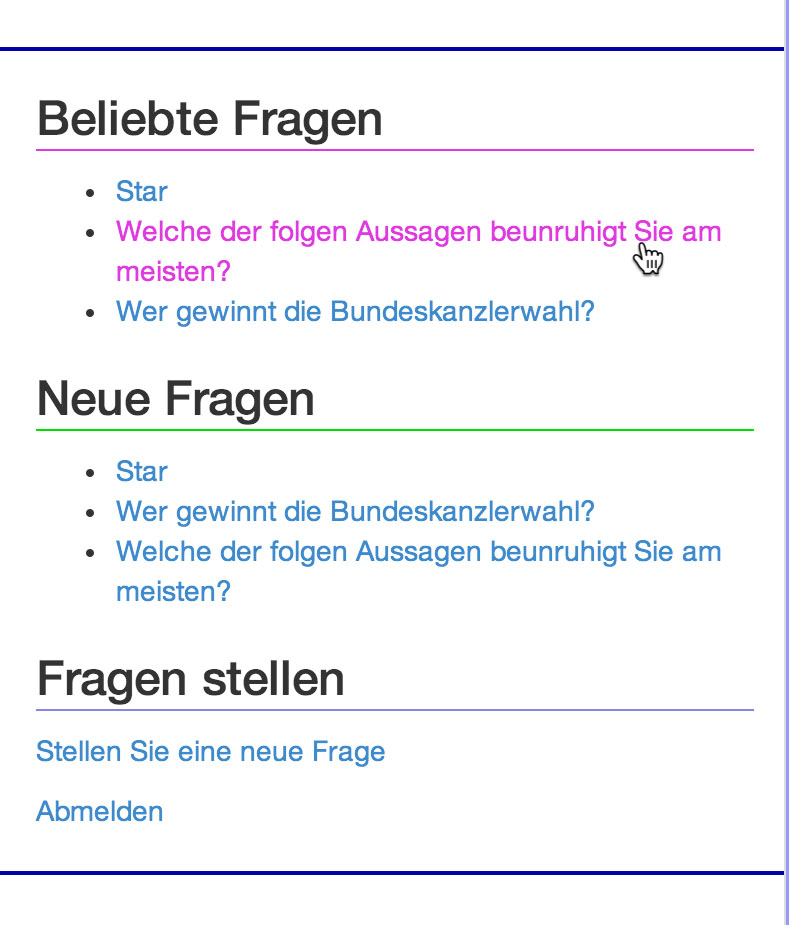
\includegraphics[width=\textwidth]{seitenleiste.jpg}
\caption{Unterstreichung und Link--Hervorhebung}
\end{center}
\label{fig:seitenleiste}
\end{figure}



\subsection{Mögliche Benutzerpfade durch die Anwendung}

Abbildung \ref{fig:zustaende} auf Seite \pageref{fig:zustaende}

\begin{figure}[h]
\begin{center}
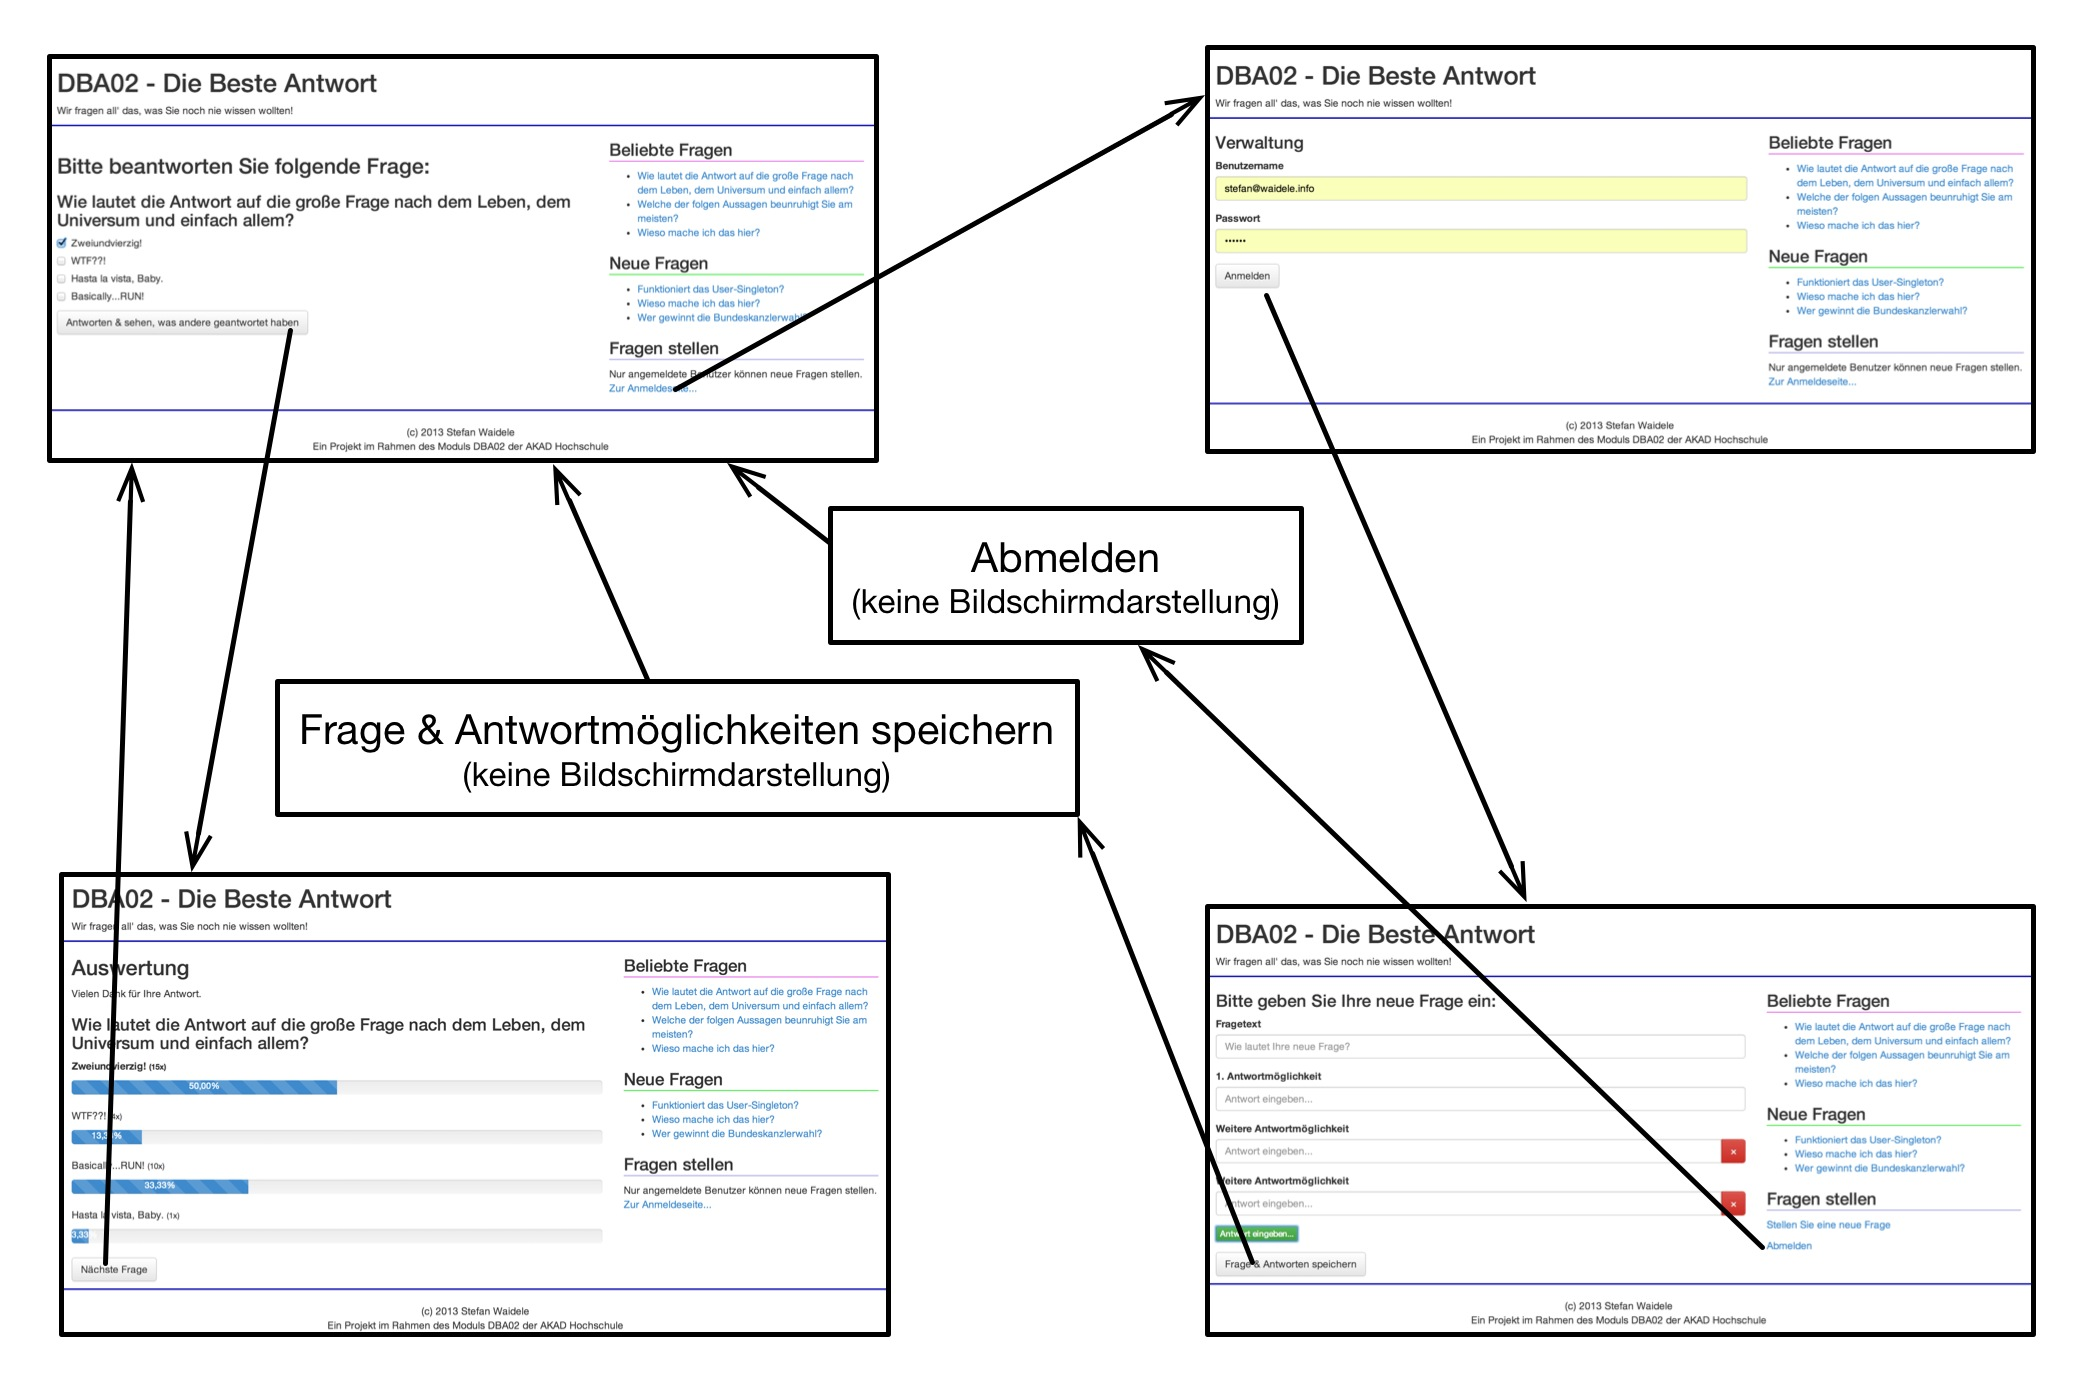
\includegraphics[width=\textwidth]{zustaende.jpg}
\caption{HTML--Seiten und Verlinkungen}
\end{center}
\label{fig:zustaende}
\end{figure}

